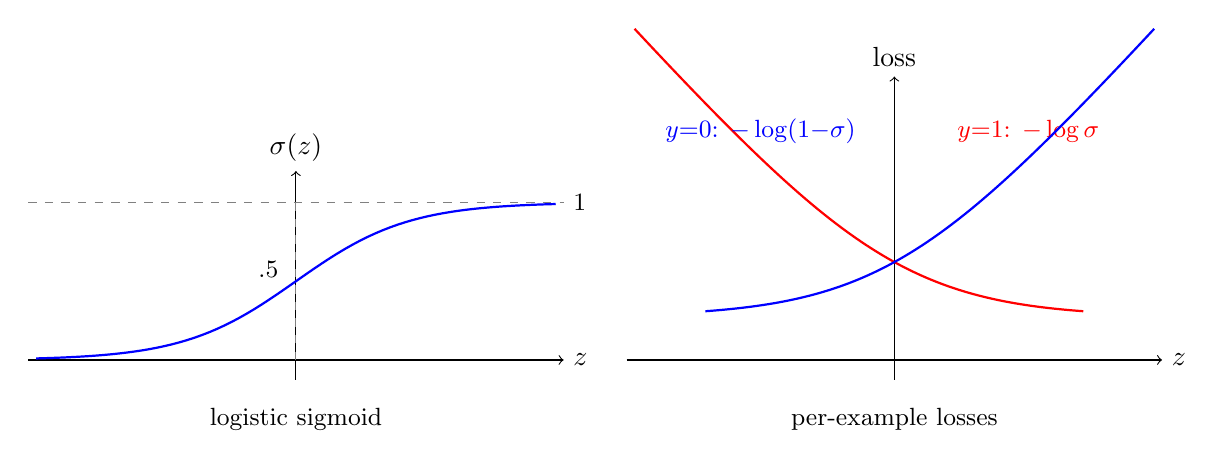
\begin{tikzpicture}[scale=1.0]
% left: sigmoid
\begin{scope}
\draw[->] (-3.4,0)--(3.4,0) node[right]{$z$};
\draw[->] (0,-0.25)--(0,2.4) node[above]{$\sigma(z)$};
\draw[dashed,gray] (-3.4,2.0)--(3.4,2.0) node[right,black,font=\small]{$1$};
\draw[dashed,gray] (0,0)--(0,2.0);
\node at (-0.35,1.15) {\small .5};
\draw[thick,blue,domain=-3.3:3.3,samples=70] plot (\x,{2.0/(1+exp(-1.4*\x))});
\node at (0,-0.75) {\small logistic sigmoid};
\end{scope}
% right: logistic loss -log(sigmoid(z)) for y=1, -log(1-s) for y=0
\begin{scope}[xshift=7.6cm]
\draw[->] (-3.4,0)--(3.4,0) node[right]{$z$};
\draw[->] (0,-0.25)--(0,3.6) node[above]{loss};
\draw[thick,red,domain=-3.3:2.4,samples=70] plot (\x,{ln(1+exp(-1.1*\x))/ln(2.71828)+0.55});
\node[red] at (1.7,2.9) {\small $y{=}1$: $-\log\sigma$};
\draw[thick,blue,domain=-2.4:3.3,samples=70] plot (\x,{ln(1+exp(1.1*\x))/ln(2.71828)+0.55});
\node[blue] at (-1.7,2.9) {\small $y{=}0$: $-\log(1{-}\sigma)$};
\node at (0,-0.75) {\small per-example losses};
\end{scope}
\end{tikzpicture}
